\chapter{核磁共振波谱}

\begin{introduction}
	\item 核磁共振的产生
	\item 核磁共振的基本概念
	\item 自旋-自旋耦合和裂分的规律(掌握)
	\item 一级谱图的解析(熟悉)
	\item 核磁共振波谱仪和样品制备(了解)
	\item $\ce{^{13}C}$谱(简要了解)
\end{introduction}

NMR的研究对象:磁性核与电磁波的相互作用。利用磁场中的磁性原子核吸收电磁波时产生的能级分裂与共振现象研究物质结构。

\section{核磁共振产生的基本条件}
%1、核磁共振产生的基本条件?
\subsection{外加磁场}
无外加磁场时,样品中的磁性核任意取向,能量相等;放入磁场中,核的磁角动量取向统一,与磁场方向平行(低能量)或反平行(高能量),产生\textbf{能量差}。

\subsection{磁性核}
\begin{definition*}{磁性核}{}
	具有磁矩的原子核称为磁性核。
	
	自旋量子数$I\neq 0$的核为磁性核,可以产生NMR信号;
	
	$I = 0$的核为非磁性核,无NMR信号。
\end{definition*}

原子核组成(质子数$p$与中子数$n$)与$I$的经验规则:
\begin{itemize}
	\item $p$与$n$同为偶数,$I = 0$。如 $\ce{^{12}C, ^{16}O, ^{32}S}$等。
	\item $p$与$n$一奇一偶,$I$为半整数(1/2,3/2,5/2等)。如$\textcolor{red}{\ce{^{1}H, ^{13}C, ^{15}N}},\ce{^{17}O, \textcolor{red}{^{31}P}}$等。
	\item $p$与$n$同为奇数,$I$为整数。如$\ce{^{2}H, ^{6}Li}$等。
	\item $I=1/2$的原子核(标为红色的几种同位素),其电荷均匀分布于原子核表面,这样的原子核不具有四极矩,其核磁共振的谱线窄,最宜于核磁共振检测。
\end{itemize}

\begin{note}
	磁距$\mu$,自旋角动量$P$,自旋量子数$I$的关系\footnote{$\gamma$是磁旋比,原子核的重要属性}:
	\begin{gather*}
		\mu=\gamma P\\
		P=\hbar \sqrt{I(I+1)}
	\end{gather*}
\end{note}

\subsection{特定频率的电磁波}
用能量等于$\Delta E$的电磁波照射磁场中的磁性核,则低能级上的某些核会被激发到高能级上去,或核自旋由与磁场平行方向转为反平行。

\begin{note}
推导:磁距$\mu_z$与磁场$B_0$的相互作用能$E$为
\begin{equation*}
	E=-\mu_zB_0=\gamma P_zB_0
\end{equation*}

原子核间进行能级跃迁的能量为\footnote{选率:$\Delta m=\pm 1$}
\begin{align*}
	\Delta E&=E_{-1/2}-E_{1/2}\\
	&=\gamma\hbar\Delta mB_0\\
	&=\gamma\hbar B_0 
\end{align*}

所以磁场固定时,不同频率的电磁波可使不同的核($\gamma$不同)产生共振;对于同样的核($\gamma$一定),改变磁场时,吸收频率不同。
\end{note}

\begin{note}
补充概念:
\begin{itemize}
	\item 弛豫过程:饱和状态(两能级间原子核数目相等)时观测不到NMR信号。要观测到净能量吸收,必须有核从高能态返回低能态,此即驰豫过程。
	\item 驰豫的两种方式:
	\begin{itemize}
		\item 自旋-晶格弛豫:高能级核返回低能级时失去能量,该能量被周围分子吸收转变成热运动。		
		\item 自旋-自旋驰豫:高能态的核把能量传给低能态的核而自己回到基态。
	\end{itemize}
	\item 谱线宽度与驰豫时间成反比。
	\item 灵敏度:
	\begin{equation*}
		N_{\alpha}/N_{\beta}\approx 1+\dfrac{\gamma\hbar B_0}{kT}
	\end{equation*}
	$N_{\alpha},N_{\beta}$分别是低、高能态核的数目。由上式可知,灵敏度与$B_0$呈线性关系。
\end{itemize}

\end{note}

\section{核磁共振的基本概念}
%2、什么是屏蔽效应?什么是化学位移?常用的基准物质是什么?熟悉常见化合物的质子位移(例如苯环上的氢、醛基氢、羧酸氢等)。
%3、什么自旋-自旋耦合和裂分?掌握自旋-自旋耦合和裂分的规律,什么是耦合常数?
\begin{definition*}{屏蔽效应}{}
	核外电子对原子核有一定的屏蔽作用,使实际作用于核的静磁感应强度不是$B_0$而是$B_0(1-\sigma)$。 
	
	$\sigma$:屏蔽系数/屏蔽常数。
\end{definition*}

\begin{definition*}{化学位移}{}
	特定质子的吸收位置与标准质子的吸收位置之差,称为该质子的化学位移,用$\delta$(ppm)表示。
	\begin{equation*}
		\delta=\dfrac{\nu_{\text{样}}-\nu_{\text{标}}}{\nu_{\text{标}}}\times 10^6 \mathrm{ppm}
	\end{equation*}
\end{definition*}

\begin{emptytcb*}{常用的基准物质}{}
	主要分两类:秃核(无屏蔽作用)或电子云密度非常大的核(屏蔽系数非常大,$\delta$=0)
	
	常见基准物质: 
	\begin{itemize}
		\item $\ce{^{1}H}$-NMR:TMS(四甲基硅烷)	
		\item $\ce{^{13}C}$-NMR:TMS
		\item $\ce{^{14}N}$-NMR:液氮		
		\item $\ce{^{17}O}$-NMR:$\ce{H2O}$
		\item $\ce{^{19}F}$-NMR:$\ce{CFCl3}$
		\item $\ce{^{31}P}$-NMR:85\%$\ce{H3PO4}$
	\end{itemize}	
\end{emptytcb*}

TMS的优势:
\begin{itemize}
	\item 由于屏蔽系数几乎比所有其他物质的都大,一般化合物$\delta$值都为正;
	\item 等价质子多,低含量的TMS可得到足够强的尖峰,且是单峰;
	\item 性质稳定,在大多数有机液体中的溶解性好,沸点低,蒸汽压高,可挥发除去,便于回收样品;
	\item 不溶于水,但对于水溶液,有DDS和TSP-d4等钠盐替代品。
\end{itemize}

\section{自旋-自旋耦合和裂分的规律}
%3、什么自旋-自旋耦合和裂分?掌握自旋-自旋耦合和裂分的规律,什么是耦合常数?

\begin{definition*}{化学位移}{}
	自旋-自旋耦合:核自旋通过成键电子与附近相邻磁性核自旋间的相互作用所引起的NMR谱线分裂现象。
	
	裂分:核磁共振谱谱峰的分裂。
\end{definition*}

\subsection{谱线分裂数的n+1规则\label{sec:n+1}}

在$\ce{H}$谱中,$n$为相邻原子上$\ce{H}$的数量。当只有一个相邻原子时,受耦合作用而产生的谱线裂分数为$n+1$\footnote{推广:分裂谱线数为$2nI+1$,$n$表示产生耦合的原子核(自旋量子数为1/2)的数目。}。

每相邻两条谱线间距离相等,谱线间强度比为$(a+b)^n$展开式的各项系数\footnote{理解:相邻碳上$n$个质子的自旋角动量叠加,每个质子有两种取向,所以总自旋角动量的绝对值可以取$n+1$个值。},如图\ref{fig:chp6split}。

有多个相邻碳原子时,对于低分辨率核磁($J$相差不大),会有$n_1+n_2+1$个峰,对于高分辨率核磁,会有$(n_1+1)\times (n_2+1)$个峰。

\begin{figure}[!h]
	\centering
	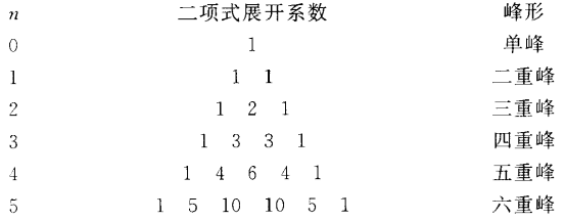
\includegraphics[width=0.7\linewidth]{image/chp6_split}
	\caption{裂分峰的强度比}
	\label{fig:chp6split}
\end{figure}

\subsection{耦合常数}

\begin{definition*}{耦合常数}{}
	耦合常数$J$:谱线裂分所产生的裂距,反映两个核之间的作用力强弱,单位Hz。与两核之间相隔的化学键数目关系很大。在$J$的左上方标以两核相距的化学键数目。
\end{definition*}

\begin{itemize}
	\item $^{2}J$:同碳上的氢,无耦合。不同种磁性核时,有耦合。
	\item $^{3}J$:相邻碳上的氢。如$\ce{H_A-CH2-CH2-H_B}$,$\ce{H_A}$与$\ce{H_B}$的耦合。
	\item $^{4}J$:相隔4个化学键,耦合作用很弱。若$J\neq 0$,则称长程耦合。
\end{itemize}

\section{一级谱图的解析}
%4、熟悉一级谱图的解析。

\subsection{一级谱图}
\begin{itemize}
	\item 满足$(\Delta \nu/J)>6$条件的谱图称为一级谱图。$\Delta \nu$为化学位移之差;$J$为耦合常数。
	\item 相同$\delta$值得几个核对任一另外的核有相同的耦合常数。
	\item (n+1)规律只适用于一级谱图:见\ref{sec:n+1}
\end{itemize}

\subsection{谱图上能获得的主要信息}
\begin{itemize}
	\item 化学位移——判断核所处的\textbf{化学环境};
	\item 耦合裂分——从峰的裂分个数及偶合常数鉴别谱图中相邻的核,以说明分子中基团间的\textbf{空间关系};
	\item 积分线——高度代表了各组峰面积,而峰面积与分子中相应的各种核的数目成正比,通过比较积分线高度可以确定各组核的\textbf{相对数目}。
\end{itemize}

\subsection{常见化合物的质子位移}

\subsubsection{烷基}
对于烷基,$\delta$值一般在0~2 ppm 。
\begin{itemize}
	\item 饱和$\ce{-CH3}$:在高场约0.9ppm出峰,峰强,在连接烷基链时易于辨认。
	\item $\ce{-CH2-}$一般较$\ce{-CH3}$大0.3ppm,$\ce{-CH-}$又较$\ce{-CH2-}$大0.3ppm
\end{itemize}

\begin{figure}
	\centering
	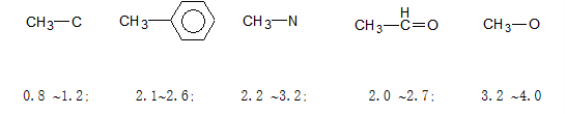
\includegraphics[width=0.7\linewidth]{image/chp6_delta1}
	\caption{甲基}
	\label{fig:chp6delta1}
	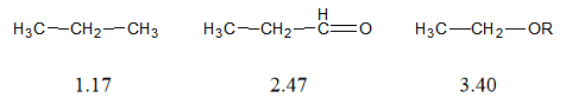
\includegraphics[width=0.7\linewidth]{image/chp6_delta2}
	\caption{亚甲基}
	\label{fig:chp6delta2}
\end{figure}

\subsubsection{烯}
$\delta$值一般在4~7 ppm(6.5 ppm左右较普遍);当双键连有卤素原子时,卤素所连碳上的另一个氢$\delta$最大,即图中的$\delta_{\ce{^{1}H_c}}$最大。

\subsubsection{苯环}
\begin{itemize}
	\item 无取代基时,$\delta_{\ce{^{1}H}}=7.3$ ppm, 单峰
	\item 烃基单取代:如$\ce{-CH3},\ce{-CH2-}$等,一组峰,分辨不开
	\item 活化基团单取代:两组高场峰,邻对位在较高场(无法分辨),间位在较低场
	\item 钝化基团单取代:两组低场峰,间对位在较高场(无法分辨),邻位在较低场
\end{itemize}

\subsubsection{醛基氢}
$\delta$值一般在9~10ppm。

\subsubsection{羧基氢}
$\delta$值一般在12+ppm。

可参考下图:
\begin{figure}[!h]
	\centering
	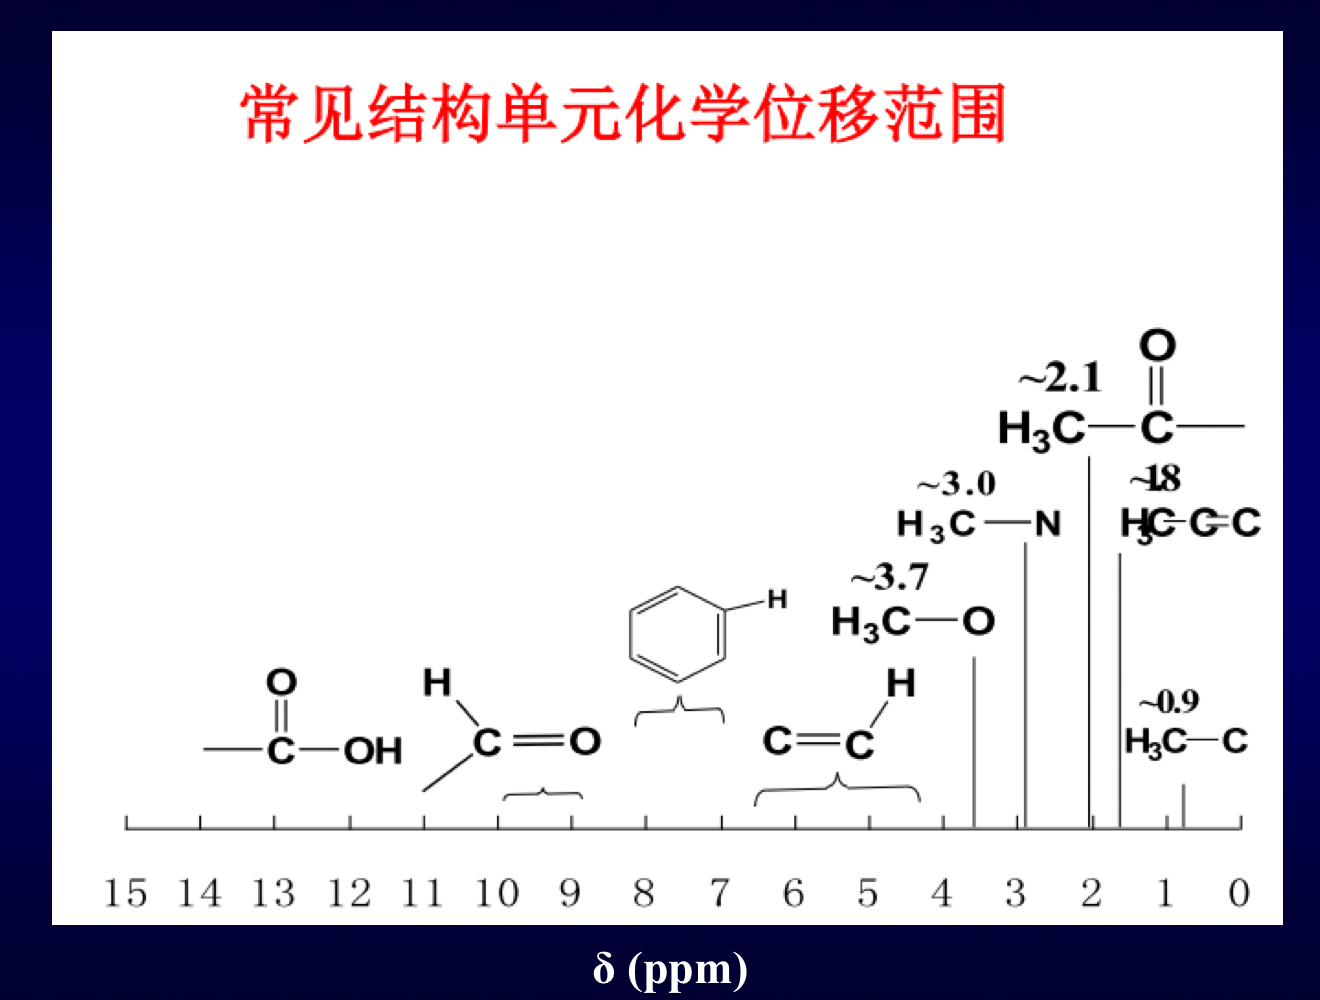
\includegraphics[width=0.6\linewidth]{image/chp6_1HNMR}
%	\caption{}
	\label{fig:chp61hnmr}
\end{figure}


需要说明化学等价的的概念:指同一个碳上的原子($\alpha$位有手性碳的不是)或在分子中处于对称(旋转轴、对称中心、对称面)位置的质子。


\subsection{化学位移的影响因素}
\subsubsection{取代基电负性—诱导效应}
取代基电负性越强,\textbf{吸电子作用越强,价电子偏离质子,屏蔽效应减弱},信号峰在低场出现。

\begin{example}
	相连碳原子的sp杂化。从$\ce{sp^3}$到$\ce{sp^2}$,s电子的成分从25\%增加到33\%,键电子更靠近碳原子,对质子有去屏蔽效应,共振位置移向低场。如图\ref{fig:chp61hnmrx}:
\begin{figure}[!h]
	\centering
	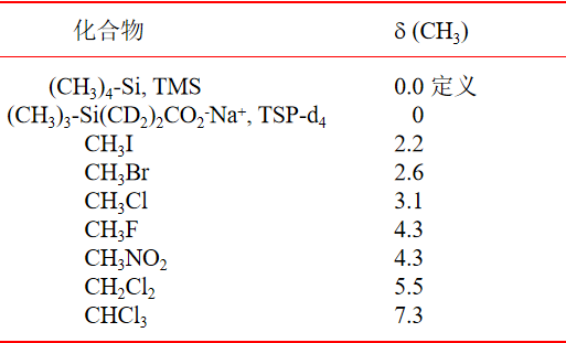
\includegraphics[width=0.5\linewidth]{image/chp6_1HNMR_X}
	\caption{诱导效应的影响}
	\label{fig:chp61hnmrx}
\end{figure}
\end{example}

\subsubsection{环电流效应}
环状共轭体系(4n+2)的离域$\pi$电子产生环电流,环电流产生的磁力线方向在苯环上下方与外磁场磁感应强度方向相反,在苯环侧面方向相同。类似物理中的楞次效应。

结果:环外氢为顺磁效应,去屏蔽,$\delta$增大;环内侧氢为逆磁效应,屏蔽,$\delta$减小。

\begin{example}
18-轮烯:环外氢$\delta$为正;环内侧氢$\delta$为负。

\begin{figure}[!h]
	\centering
	\subfigure[环电流]{
		\begin{minipage}[t]{0.42\linewidth}
			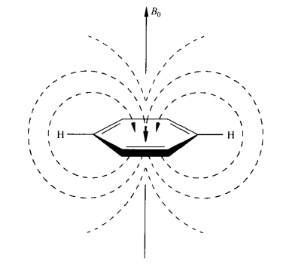
\includegraphics[width=\textwidth]{chp6_benzene}
	\end{minipage}}
	\quad
	\subfigure[18-轮烯]{
		\begin{minipage}[t]{0.42\linewidth}
			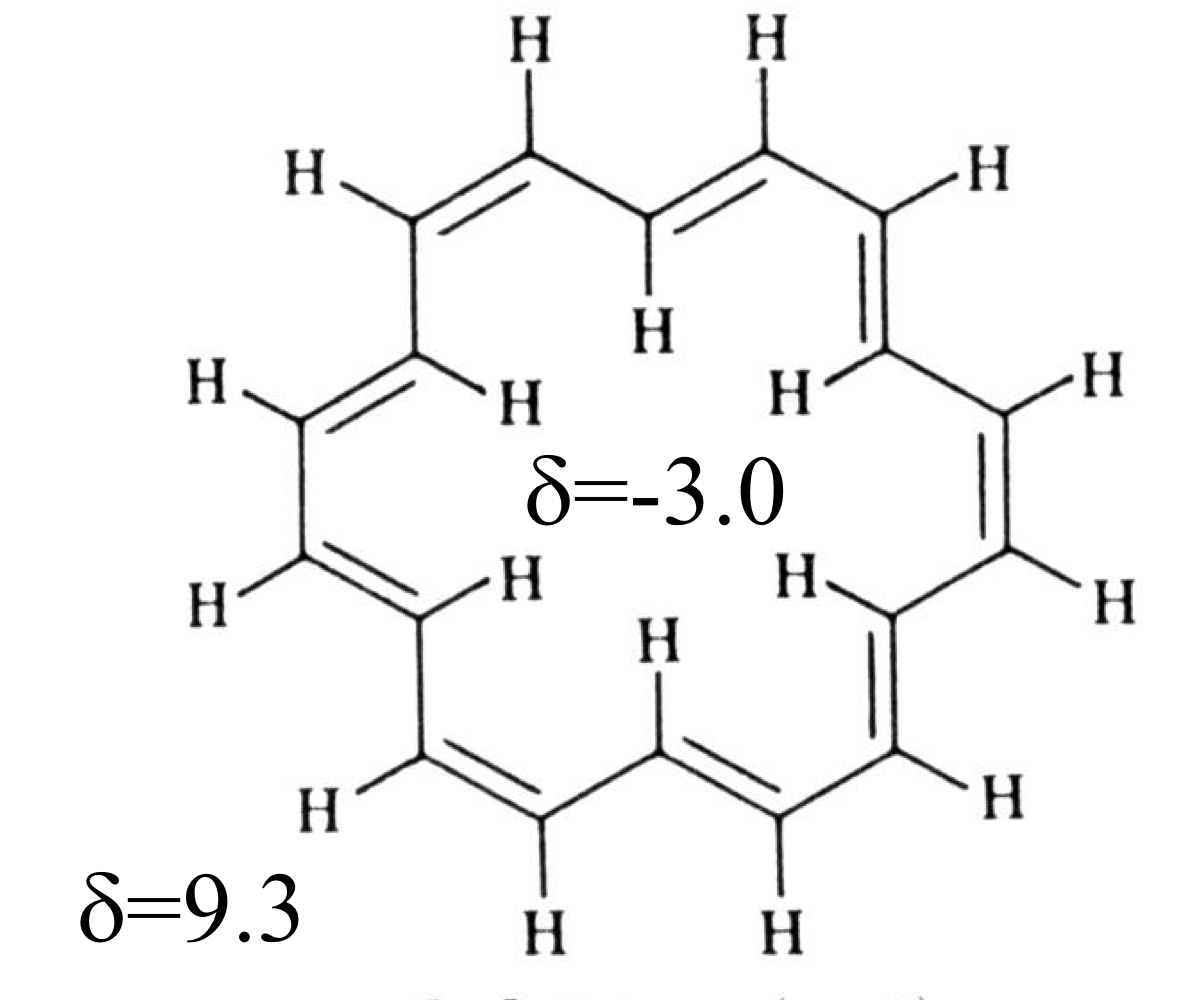
\includegraphics[width=\textwidth]{chp6_18}
	\end{minipage}}
\end{figure}

\end{example}

\subsubsection{相邻键的磁各向异性}
一般的,三键电子云磁感应强度与键轴共线,而双键电子云产生的磁感应强度则与分子平面垂直。
\begin{figure}[!h]
	\centering
	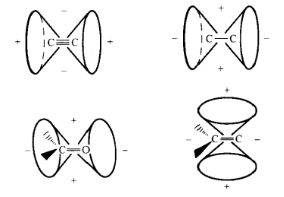
\includegraphics[width=0.6\linewidth]{image/chp6_doubletriplebond}
%	\caption{}
	\label{fig:chp6doubletriplebond}
\end{figure}

\begin{itemize}
	\item 双键C上的氢受去屏蔽作用,$\delta$值高于饱和C;
	\item 叁键C上的氢受屏蔽作用,$\delta$减小。
\end{itemize}

\subsubsection{其他作用}
电偶极和范德华力,介质,氢键等。

\section{核磁共振波谱仪}
%5、了解核磁共振波谱仪的基本组成及各部分功能,了解样品的制备。

\subsection{基本组成及功能}
\subsubsection{外加磁场}
强弱的表示:磁场强度$B_0$,单位:$\mathrm{T}$。
不过习惯用氢核的共振频率来表示。
	如100M的仪器,$B_0=2.35\mathrm{T}$。

要求:强而稳定、均匀

磁铁:分为永久磁铁、电磁铁和超导磁铁。

性能影响因素:
\begin{itemize}
	\item 磁场强度越强,低能级上核的数目越多,灵敏度越高。
	\item 磁场越强,以频率表示的化学位移越大,分辨率越高。
	\item 磁场的均一性越好,分辨率越高。
\end{itemize}

\subsubsection{探头}
呈圆柱形,安装于在磁体中心。作用:对样品管发射脉冲电磁波,检测核磁共振信号。

分类:
\begin{itemize}
	\item 产生固定频率的探头
	\begin{itemize}
		\item 双核探头($\ce{^{1}H,^{13}C}$)
		\item 四核探头($\ce{^{1}H,^{13}C,^{15}N,^{31}P}$)
	\end{itemize}
	\item 频率连续可调探头:如$\ce{^{15}N}$和$\ce{^{31}P}$。
\end{itemize}

\subsubsection{高频电磁波发生器及接受器}
\begin{itemize}
	\item 连续波NMR仪器(CW-NMR)——最简单
	\begin{itemize}
		\item 有两种扫描方式。扫频方式:固定$B_0$,扫描电磁波频率$\nu$;扫场方式:固定$\nu$,扫描磁场强度$B_0$。
		\item 不足:连续变化一个参数使不同基团的核依次满足共振条件,任一瞬间只有一种原子核处于共振状态,其它核处于等待状态。样品利用率低,灵敏度低,分辨率低。
	\end{itemize}
	\item 傅里叶变换NMR(FT-NMR)
	\begin{itemize}
		\item 磁场强,产生强而短的脉冲(高频脉冲)。在这一脉冲下,所有的核都发生共振。脉冲停止后,这些核都产生相应的核磁共振信号。这些信号含多种频率,总信号是多种频率信号的叠加,这些信号以时间为变量,也是随时间衰减的。因此,信号是时间的函数(时域谱),通过FT转换变为频域谱。
		\item 优点:所有的核同时共振;灵敏度高,样品用量少;测定时间短,可多次去平均能降低噪声。
	\end{itemize}
\end{itemize}

\subsubsection{数据处理及记录部分}

\subsection{样品制备技术}
\begin{itemize}
	\item 样品要制成粘度不高的液态:2-15\%的溶液
	\item NMR溶剂不应含氢,可用卤化或氘代溶剂,如$\ce{CDCl3, C6D6}$等。
\end{itemize}


\section{$\ce{^{13}C}$谱}
%6、简要了解碳-13谱,和氢谱相比,有什么特点?
$\ce{^{13}C}$的自然丰度约为1\%,即样品中所有$\ce{C}$只约有1\%是$\ce{^{13}C}$。由于分子数是巨大的,而原子的分布是随机的,所以可以认为分子中每个碳原子都有1\%几率是$\ce{^{13}C}$,这样就可测得代表整个分子的$\ce{^{13}C}$MR。由于$\ce{^{13}C}$自然丰度低,$\ce{^{13}C}$MR的相对灵敏度仅为氢谱的1/5600。
特点:
\begin{itemize}
	\item 碳的δ值范围0~230ppm。因为$\ce{C}$外层$\ce{p}$电子云密度变化范围大,对$\ce{C}$核的屏蔽效应变化范围也大。因此其信号不像PMR那样容易重叠,往往分子中有几个不同类$\ce{C}$,就有几组峰,能直接提供有机物碳骨架的信息。
	\item $\ce{^{13}C}$MR没有积分曲线。峰的强度与$\ce{C}$个数无关,却正比于碳上所连的$\ce{H}$数。在$\ce{^{13}C}$MR中,只提供有几类$\ce{C}$的信息,没有提供各类$\ce{C}$的相对比例。
	\item $\ce{^{13}C}$和$\ce{H}$有耦合:耦合的碳谱很乱,很难解析必须把$\ce{^{13}C}$与$\ce{^{1}H}$的偶合裂分峰去掉才行。(可以采用不同的技术进行测定)
\end{itemize}


\section{解谱例题}

\begin{example}
	某化合物分子式为$\ce{C9H12O}$,其$\ce{^{1}H}$ NMR谱如下,推测该化合物的结构。
	
	\begin{figure}[!h]
		\centering
		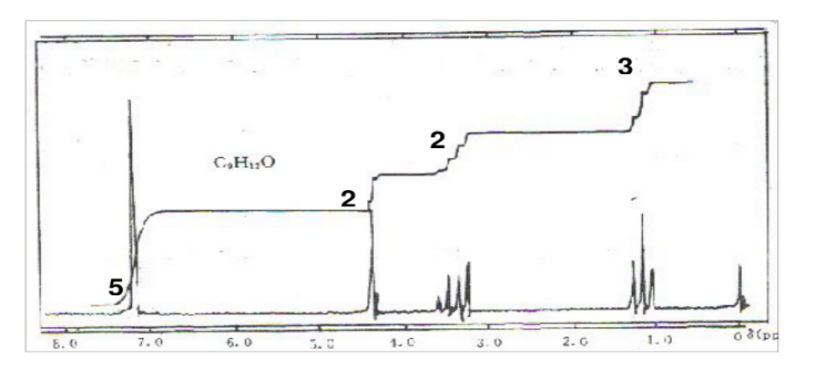
\includegraphics[width=0.9\linewidth]{image/chp6_example1}
%		\caption{}
		\label{fig:chp6example1}
	\end{figure}

	\solve
	不饱和度为4,$\delta=7.2$左右的是单取代苯的峰,所以没有其他双键和环,又无醇羟基峰,考虑醚类;3氢的三重峰和2氢的四重峰对应乙基,后者化学位移大,可能与氧相连;剩下的2氢单峰化学位移更大,可能还和苯环相连。综上,最可能是苯甲醇乙醇醚。
	\begin{figure}[!h]
		\centering
		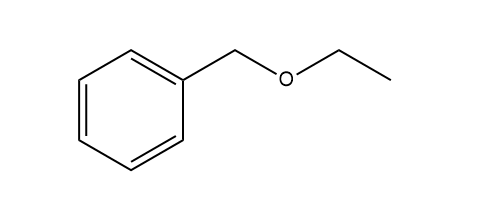
\includegraphics[width=0.6\linewidth]{image/chp6_answer1}
%		\caption{}
		\label{fig:chp6answer1}
	\end{figure}
\end{example}

\begin{example}
	某化合物分子式为$\ce{C8H8O2}$,其$\ce{^{1}H}$ NMR谱如下,推测该化合物的结构。
	
	\begin{figure}[!h]
		\centering
		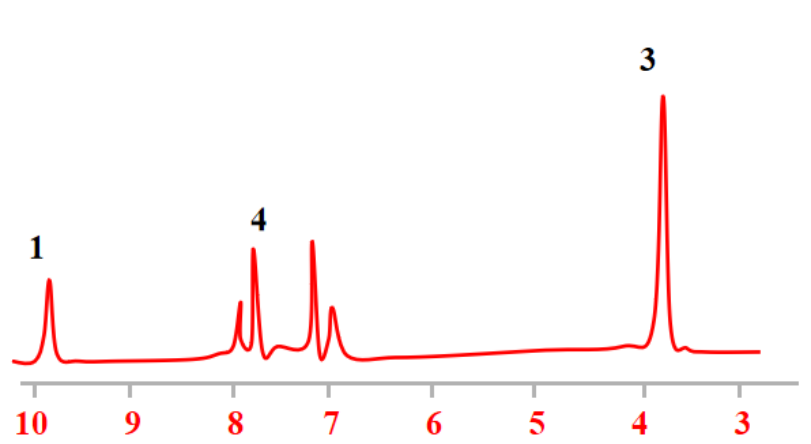
\includegraphics[width=0.7\linewidth]{image/chp6_example2}
%		\caption{}
		\label{fig:chp6example2}
	\end{figure}
	
	\solve	
	不饱和度为5,$\delta=7\sim 8$是芳环上氢,四个峰对位取代;$\delta=9.87$是醛基上氢,低场;$\delta=3.87$是$\ce{-CH3}$峰,向低场位移,与电负性基团相连,所以可能的结构是
	
	\begin{figure}[!h]
		\centering
		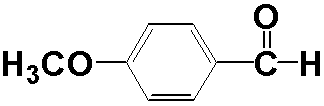
\includegraphics[width=0.5\linewidth]{image/chp6_answer2}
%		\caption{}
		\label{fig:chp6answer2}
	\end{figure}
\end{example}